% ******************************* Thesis Appendix B ********************************

\chapter{Supporting information: Chapter 4} 

\graphicspath{{Appendix3/Figs/}}

\section{Phylogeny construction details}

The community phylogeny was constructed using the program phyloGenerator (Pearse and Purvis 2013) and its dependency programs as follows. DNA sequence data for two commonly used plastid gene regions (rbcL and matK) was searched for on GenBank (Benson et al. 2011). Of the 49 taxa in the pool, 30 species were represented, with a further 16 represented by congeneric taxa. Sequences were aligned using MAFFT (Katoh et al. 2005), and the community phylogeny (with divergence times) was estimated under a Bayesian framework using BEAST (Drummond and Rambaut 2007). A constraint tree, generated in Phylomatic (Webb and Donoghue 2005), and dated using the BLADJ algorithm of Phylocom (Webb, Ackerly, and Kembel 2008), was used to place strong priors on the ages and topology of existing highly supported clades. Four independent runs were performed using a GTR model assuming a lognormal relaxed clock with four rate categories, with each run comprising an MCMC chain run for 50,000,000 generations and sampled every 1,000 generations. After checking parameter statistics in TRACER (http://tree.bio.ed.ac.uk/software/tracer/) and removing burnins of 10-20\%, the four independent runs were combined to generate a maximum clade credibility tree. Those taxa represented by congeners were then manually added to the tree, as were the three unrepresented taxa on the basis of their position on the Phylomatic derived constraint tree. 

\newpage

\textbf{Phylogeny for all 49 species in Newick tree format}

\footnotesize((((Gonocarpus micranthus: 32.78964725, Gonocarpus tetragynus: 32.78964725): 124.9441371, ((((Drosera peltata: 19.27769113, Drosera auriculata: 19.27769113): 19.27769113, Drosera pygmaea: 38.55538226): 73.73868839, Drosera spatulata: 112.2940706): 20.52500615, (Stylidium lineare: 112.3064351, (Goodenia stelligera: 74.95393085, Goodenia dimorpha: 74.95393085): 37.35250429): 20.51264166): 24.91470752): 35.6884448, (Burchardia umbellata: 150.2255016, (((((Hypolaena fastigiata: 45.02808262, (((Baloskion gracile: 23.43160533, Eurychorda complanata: 23.43160533): 6.005965644, (Empodisma minus: 12.79282614, Leptocarpus tenax: 12.79282614): 16.64474484): 9.335195904, Lepyrodia scariosa: 38.77276688): 6.25531574): 14.99415044, ((((Plinthanthesis paradoxa: 14.96742327, Aristida warburgii: 14.96742327): 10.6327861, (Themeda australis: 10.795227, Entolasia stricta: 10.795227): 14.80498236): 12.42401627, Tetrarrhena turfosa: 38.02422563): 7.018168824, Austrostipa pubescens: 45.04239445): 14.9798386): 16.64744303, (((Tricostularia pauciflora: 42.6973992, ((Lepidosperma neesii: 11.2529451, Tetraria capillaris: 11.2529451): 18.2730358, (Ptilothrix deusta: 12.26655391, (Schoenus brevifolius: 6.133276955, Schoenus ericetorum: 6.133276955, Schoenus imberbis: 6.133276955, Schoenus lepidosperma: 6.133276955, Schoenus moorei: 6.133276955): 6.133276955): 17.25942698): 13.17141831): 13.29991705, Cyathochaeta diandra: 55.99731626): 10, Xyris gracilis: 65.99731626): 10.67235984): 38.0120084, Haemodorum corymbosum: 114.6816845): 14.17530244, ((Blandfordia nobilis: 105.2018214, (((Thysanotus juncifolius: 31.32190603, (Sowerbaea juncea: 15.35052634, (Lomandra obliqua: 7.67526317, (Lomandra glauca: 4, Lomandra cylindrica: 4): 3.67526317): 7.67526317): 15.97137969): 15.40653782, (Xanthorrhoea resinosa: 31.31985316, (Thelionema umbellatum: 15.65992658, Caesia parviflora: 15.65992658): 15.65992658): 15.40859068): 28.21501178, (Patersonia sericea: 46.94615343, Patersonia fragilis: 46.94615343): 27.9973022): 30.25836574): 9.576595384, (Prasophyllum brevilabre: 106.9427746, Cryptostylis subulata: 106.9427746): 7.835642119): 14.07857018): 21.36851467): 43.1967275): 1.625295448, (Cassytha glabella: 24.29827518, Cassytha pubescens: 24.29827518): 170.7492493);


\normalsize
\subsubsection*{References}

Pearse, W. D. \& Purvis, A. 2013 phyloGenerator: an automated phylogeny generation tool for ecologists. Methods in Ecology and Evolution, 4(7), 692-698.

Drummond, A. J. \& Rambaut, A. 2007 BEAST: Bayesian evolutionary analysis by sampling trees. BMC evolutionary biology, 7(1), 214.

Benson, D. A., Karsch-Mizrachi, I., Lipman, D. J., Ostell, J. \& Sayers, E. W.
GenBank. Nucleic acids research, 39(Database issue), D32-7.

Katoh, K., Kuma, K.-i., Toh, H. \& Miyata, T. 2005 MAFFT version 5: im648
provement in accuracy of multiple sequence alignment. Nucleic acids research,
33(2), 511-8.

Webb, C. O. \& Donoghue, M. 2005 Phylomatic: tree assembly for applied
phylogenetics. Molecular Ecology Notes, 5(1), 181-183.

Webb, C. O., Ackerly, D. D. \& Kembel, S. W. 2008 Phylocom: soft654
ware for the analysis of phylogenetic community structure and trait evolution. Bioinformatics (Oxford, England), 24(18), 2098-100.

\section{Equations for calculating \textit{D}$_{nn}$ and \textit{D}$_{pw}$}

Phylogenetic and functional nearest-neighbour dissimilarity (\textit{D}$_{nn}$, the beta diversity analogue of MNTD) is given by:

$$D_{nn} = f_{A}\sum_{i=1}^{S_{A}}f_{i} min \delta _{ib} + f_{B}\sum_{j=1}^{S_{B}}f_{j}min \delta _{jb}$$

where \textit{SA} is the number of species in the community at time A, \textit{SB} is the number of species in the community at time B, $\mathrm{min \delta _{\mathit{ib}}}$ is the phylogenetic or functional distance of species \textit{i} at time B to its nearest neighbour at time A, $\mathrm{min \delta _{\mathit{ja}}}$ is the phylogenetic or functional distance of species \textit{j} at time B to its nearest neighbour at time A, $\mathit{f_{i}}$  is the relative abundance of species \textit{i} in the community at time A, and finally $\mathit{f_{j}}$ is the relative abundance of species \textit{j} in the community at time B. 

Similarly, pairwise dissimilarity (\textit{D}$_{pw}$, the beta diversity analogue of MPD) is given by:

$$D_{pw} = f_{A}\sum_{i=1}^{S_{A}}f_{i}\overline{\delta _{ib}} + f_{B}\sum_{j=1}^{S_{B}}f_{j}\overline{\delta _{ja}}$$

where terms shared with \textit{D}$_{nn}$ are equivalent, and $\overline{\delta _{ib}}$ is the mean pairwise phylogenetic or functional distance between species i in the community at time A and all species in the community at time B, and $\overline{\delta _{jb}}$ is the mean pairwise phylogenetic of functional distance between species j in the community at time B and all species in the community at time A. Note that as for MNTD and MPD, phylogenetic distance was first square-root transformed before input into both \textit{D}$_{nn}$ and \textit{D}$_{pw}$.

\subsubsection*{References}

Ricotta, C. \& Burrascano, S. 2009 Testing for differences in beta diversity
with asymmetric dissimilarities. Ecological Indicators, 9(4), 719-724.

Swenson, N. G., Stegen, J. C., Davies, S. J., Erickson, D. L., Forero-Monta~na,
J., Hurlbert, A. H., Kress, W. J., Thompson, J., Uriarte, M. et al. 2012
Temporal turnover in the composition of tropical tree communities: functional
determinism and phylogenetic stochasticity. Ecology, 93(3), 490-499.

\section{Phylogenetic signal in traits}


\footnotesize Table S4.1. Phylogenetic signal in functional traits quantified using either Blomberg's \textit{K} statistic for continuously defined traits or the `Fixed Tree, Character Randomly Reshuffled' model of Maddison \& Slatkin (1991) for traits coded ordinally.
\begin{table}[H]
\centering
\begin{tabular}{lcc}
\hline Trait & \textit{K} statistic & p-value\\
\hline log$_{10}$(seed weight)
 & 0.385 & 0.001 \\ 
log$_{10}$(maximum height)
 & 0.647 & 0.001 \\ 
Fire response & - & $<$ 0.001 \\ 
Raunki\ae r life-form
 & - & 0.005 \\ 
Fecundity & - & 0.003 \\ 
Longevity
 & - & $<$ 0.001 \\ 
Seedbank persistence
 & - & $<$ 0.001 \\ 
\hline 
\end{tabular} 
\end{table}

\pagebreak

\section{Temporal change in phylogenetic and functional community structure: supplementary figures}
\sectionmark{Temporal change in community structure: supp. figs.}

The following figures, which correspond with Figure 2 in the main article, show phylogenetic and functional community structure through time when the species pool is constrained to only include monocots or only Polaes. Trendlines correspond to models of MNTD/MPD/F-MNTD/F-MPD vs. time for all plots/sites through the first four years of sampling (solid line); plots/sites that only burnt in 1994 (dashed line) and plots that burnt in 1994 and 2001 (dotted lines). Trend lines shaded black indicate significant slope coefficients at p $<$ 0.05; grey lines indicate insignificant slopes.

\begin{figure}[H]
\centering
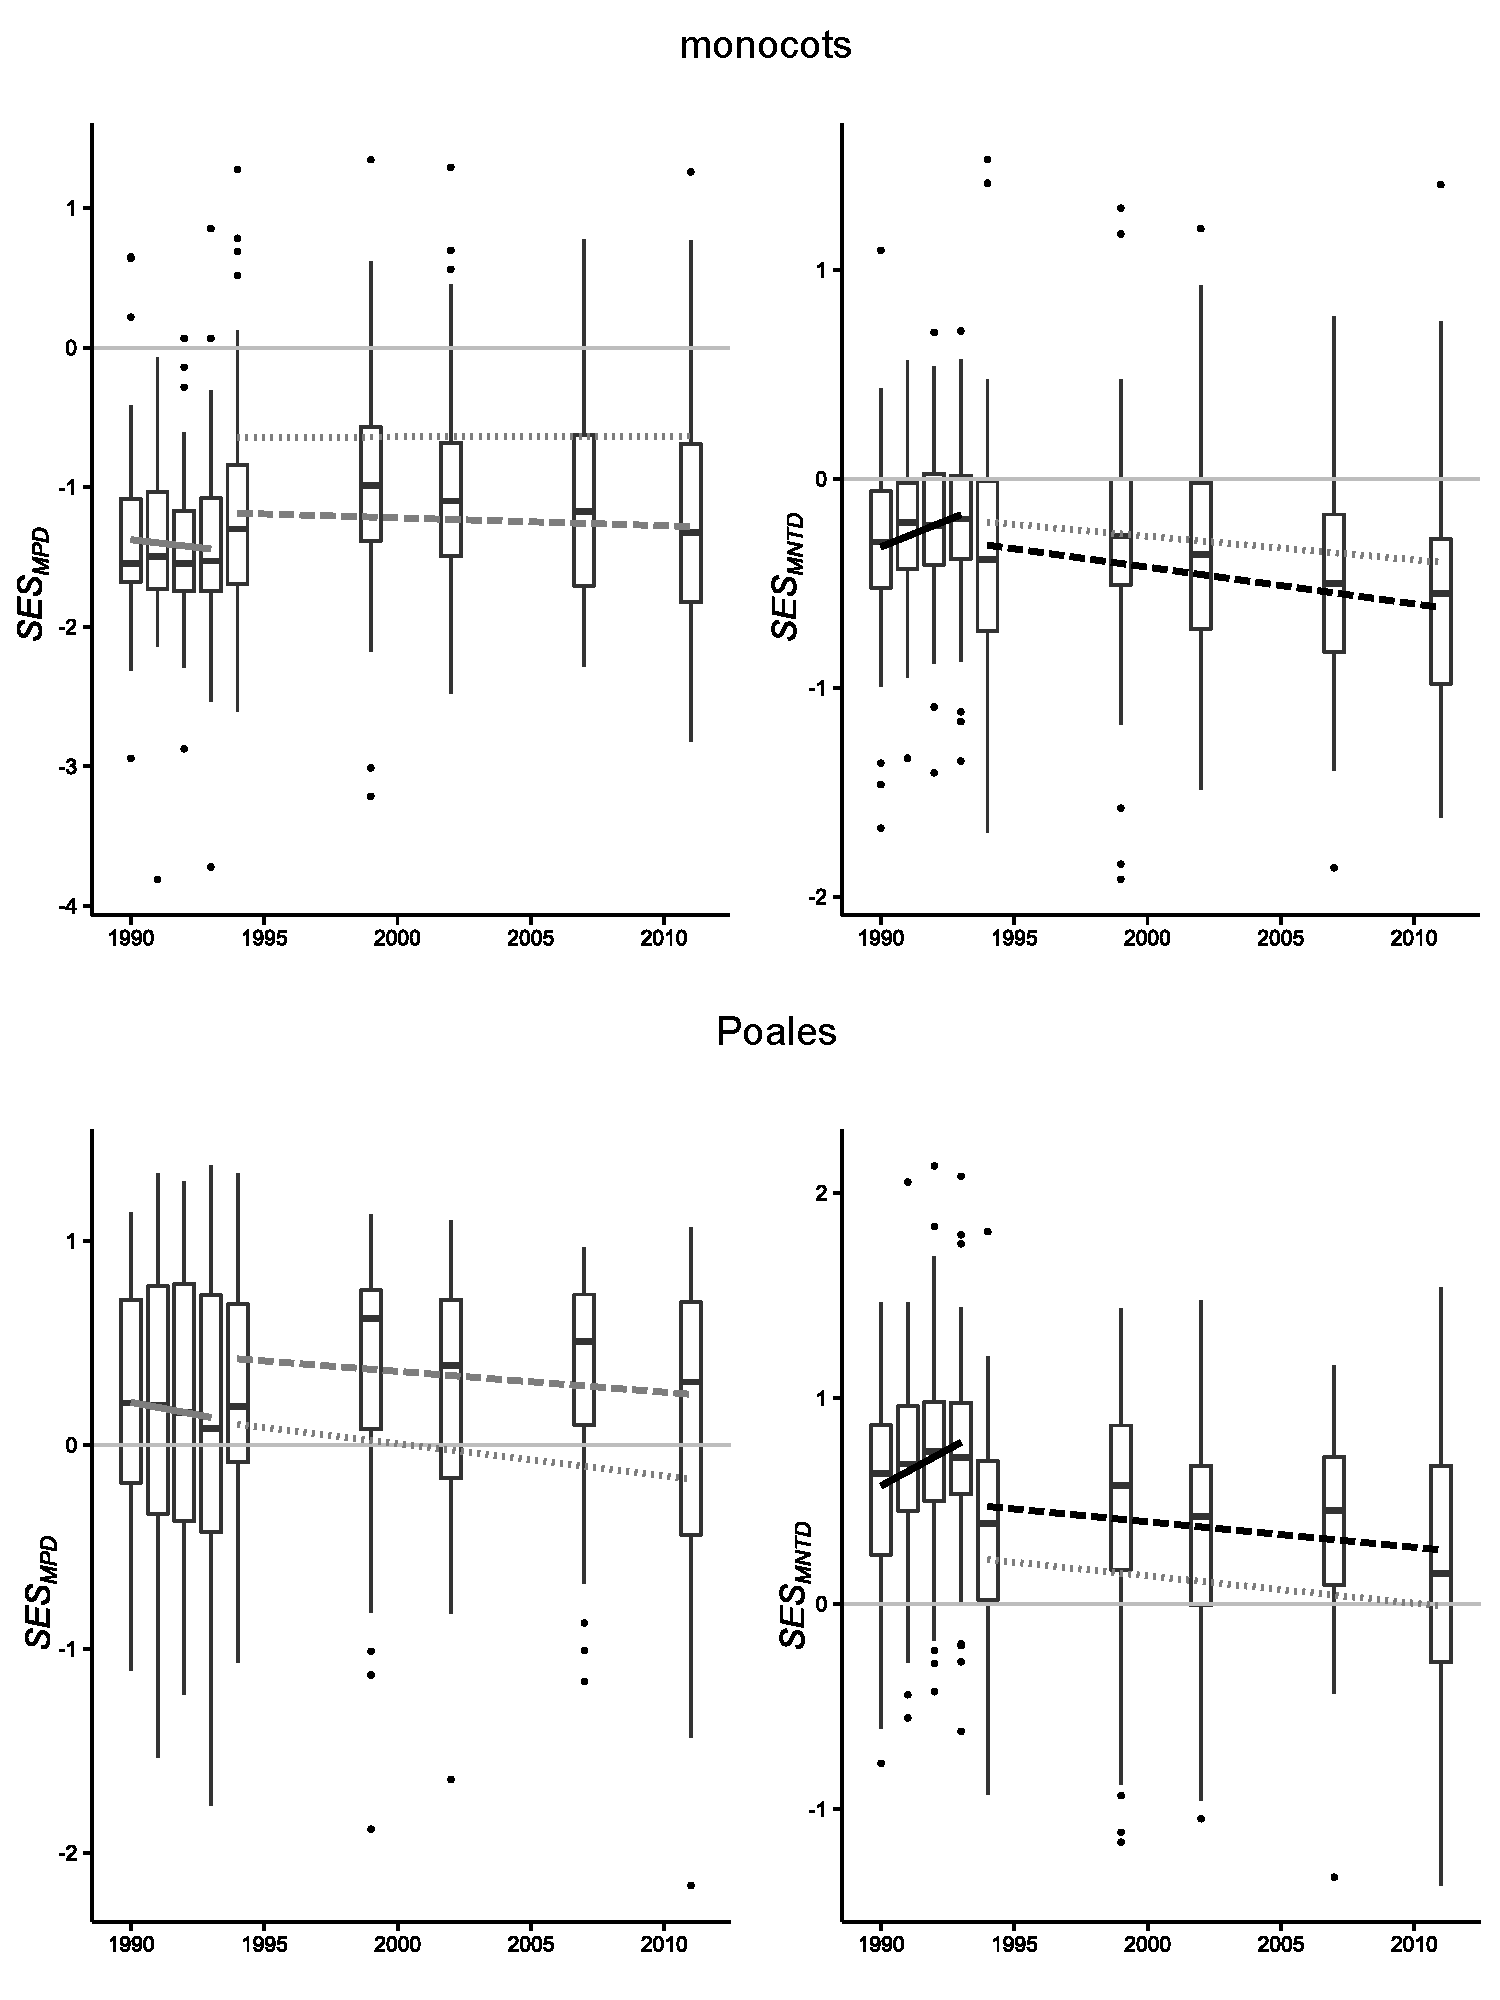
\includegraphics[width=0.7\linewidth]{phy_poales_mono_alphadiv}\\
\footnotesize Figure S4.1. Phylogenetic community structure of monocots and Poales through time at the plot scale.
\end{figure}

\begin{figure}[H]
\centering
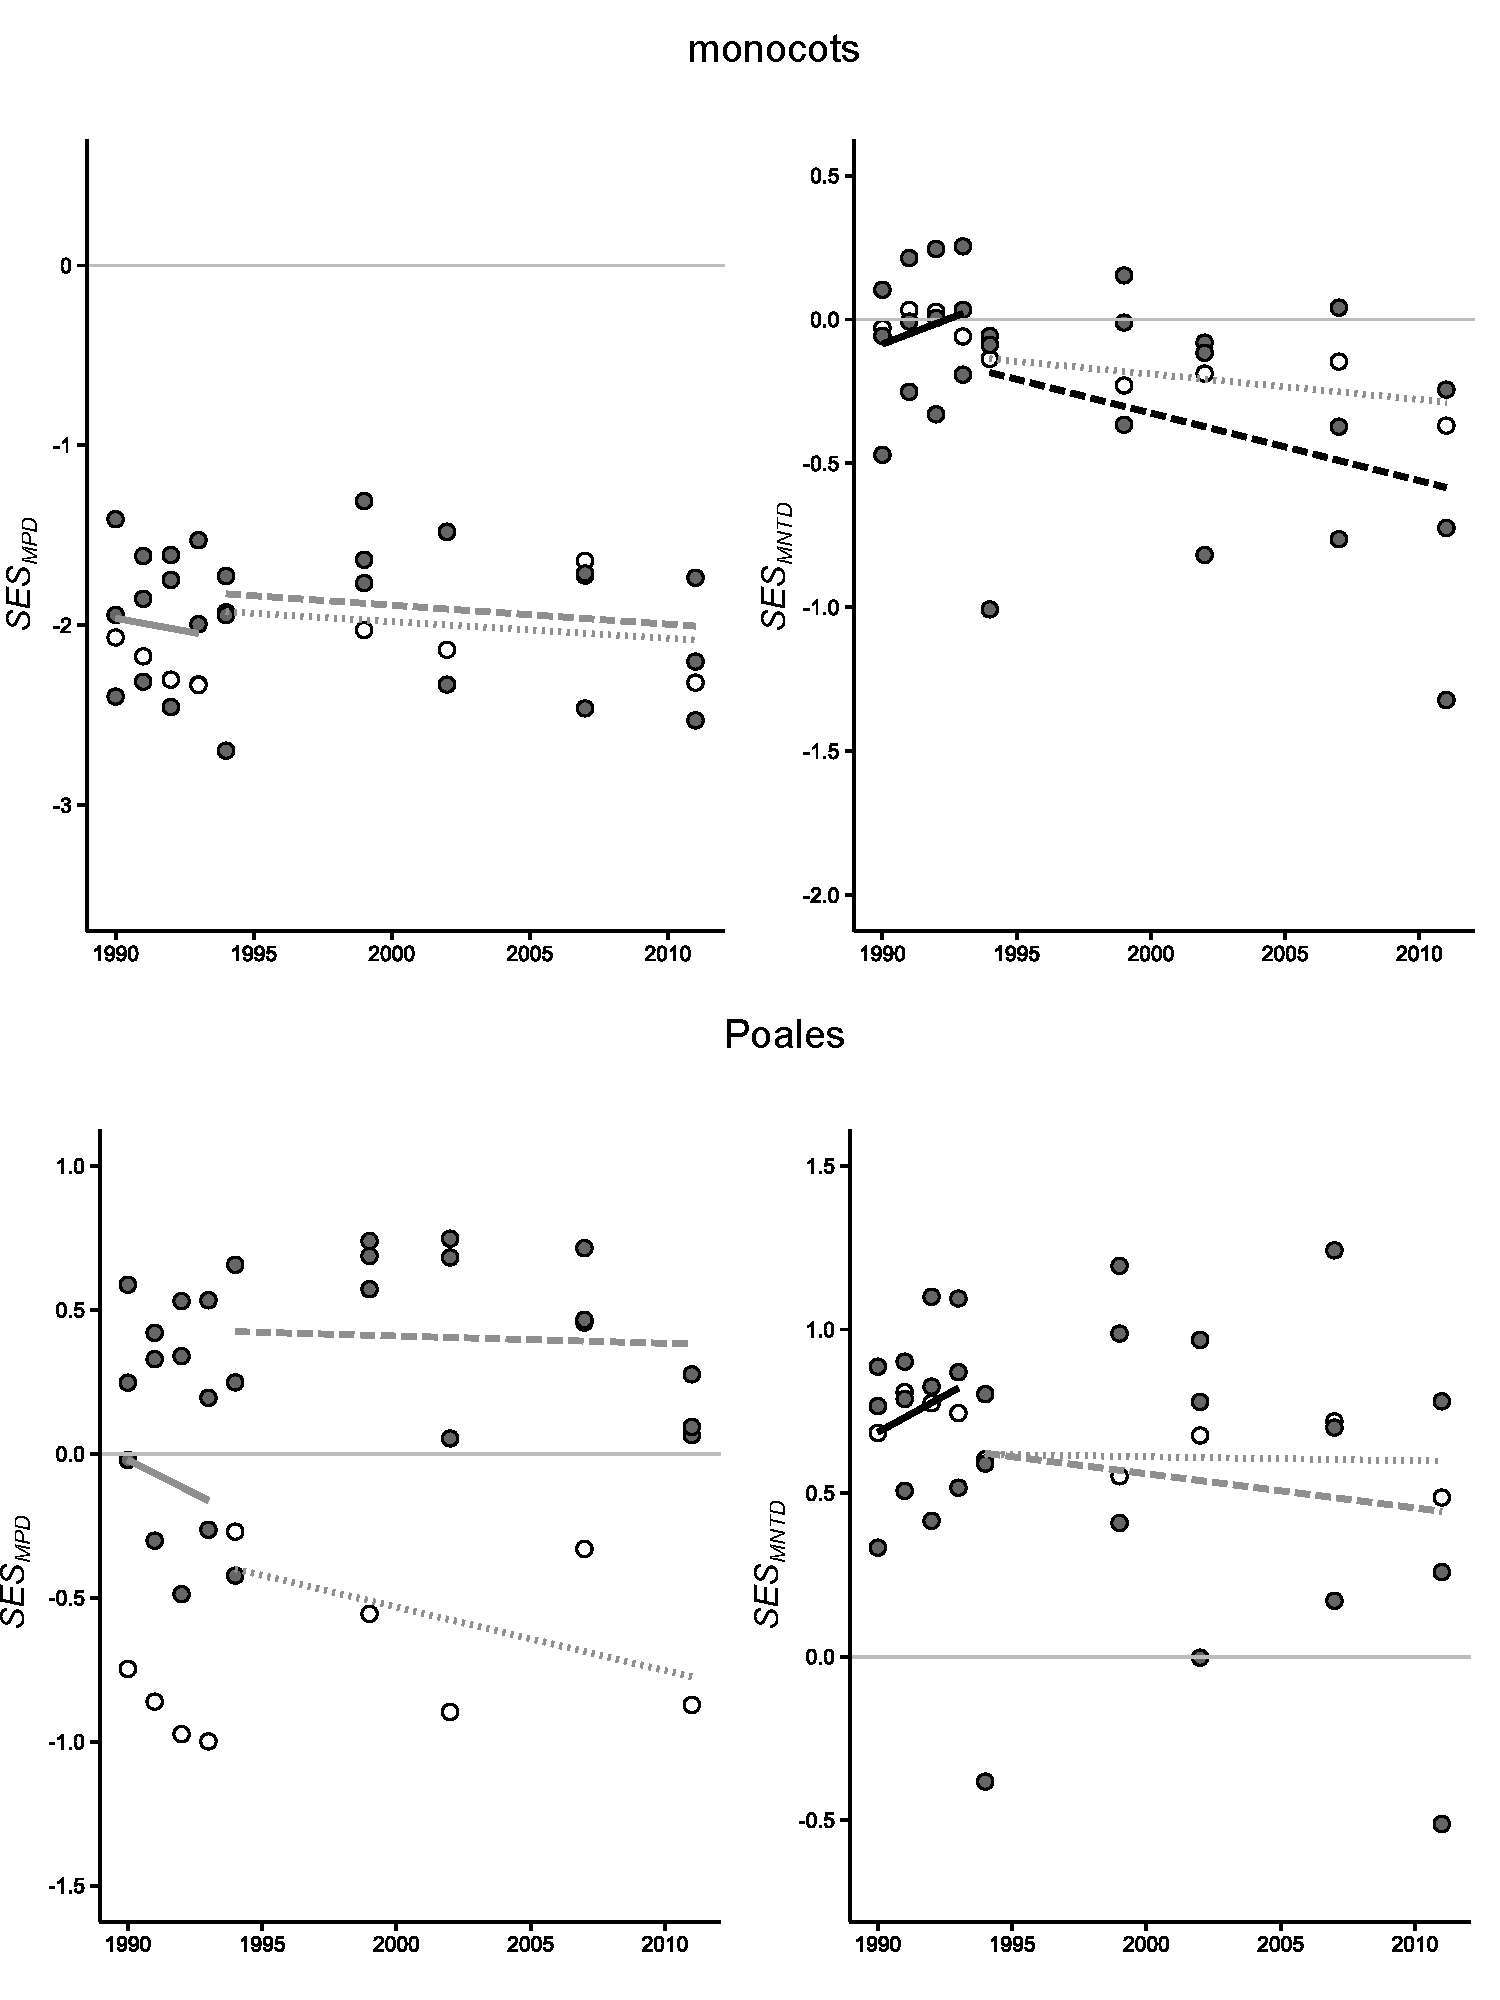
\includegraphics[width=0.7\linewidth]{phy_poales_mono_alphadiv_transectscale_points}\\
\footnotesize Figure S4.2. Phylogenetic community structure of monocots and Poales through time at the site scale.
\end{figure}

\begin{figure}[H]
\centering
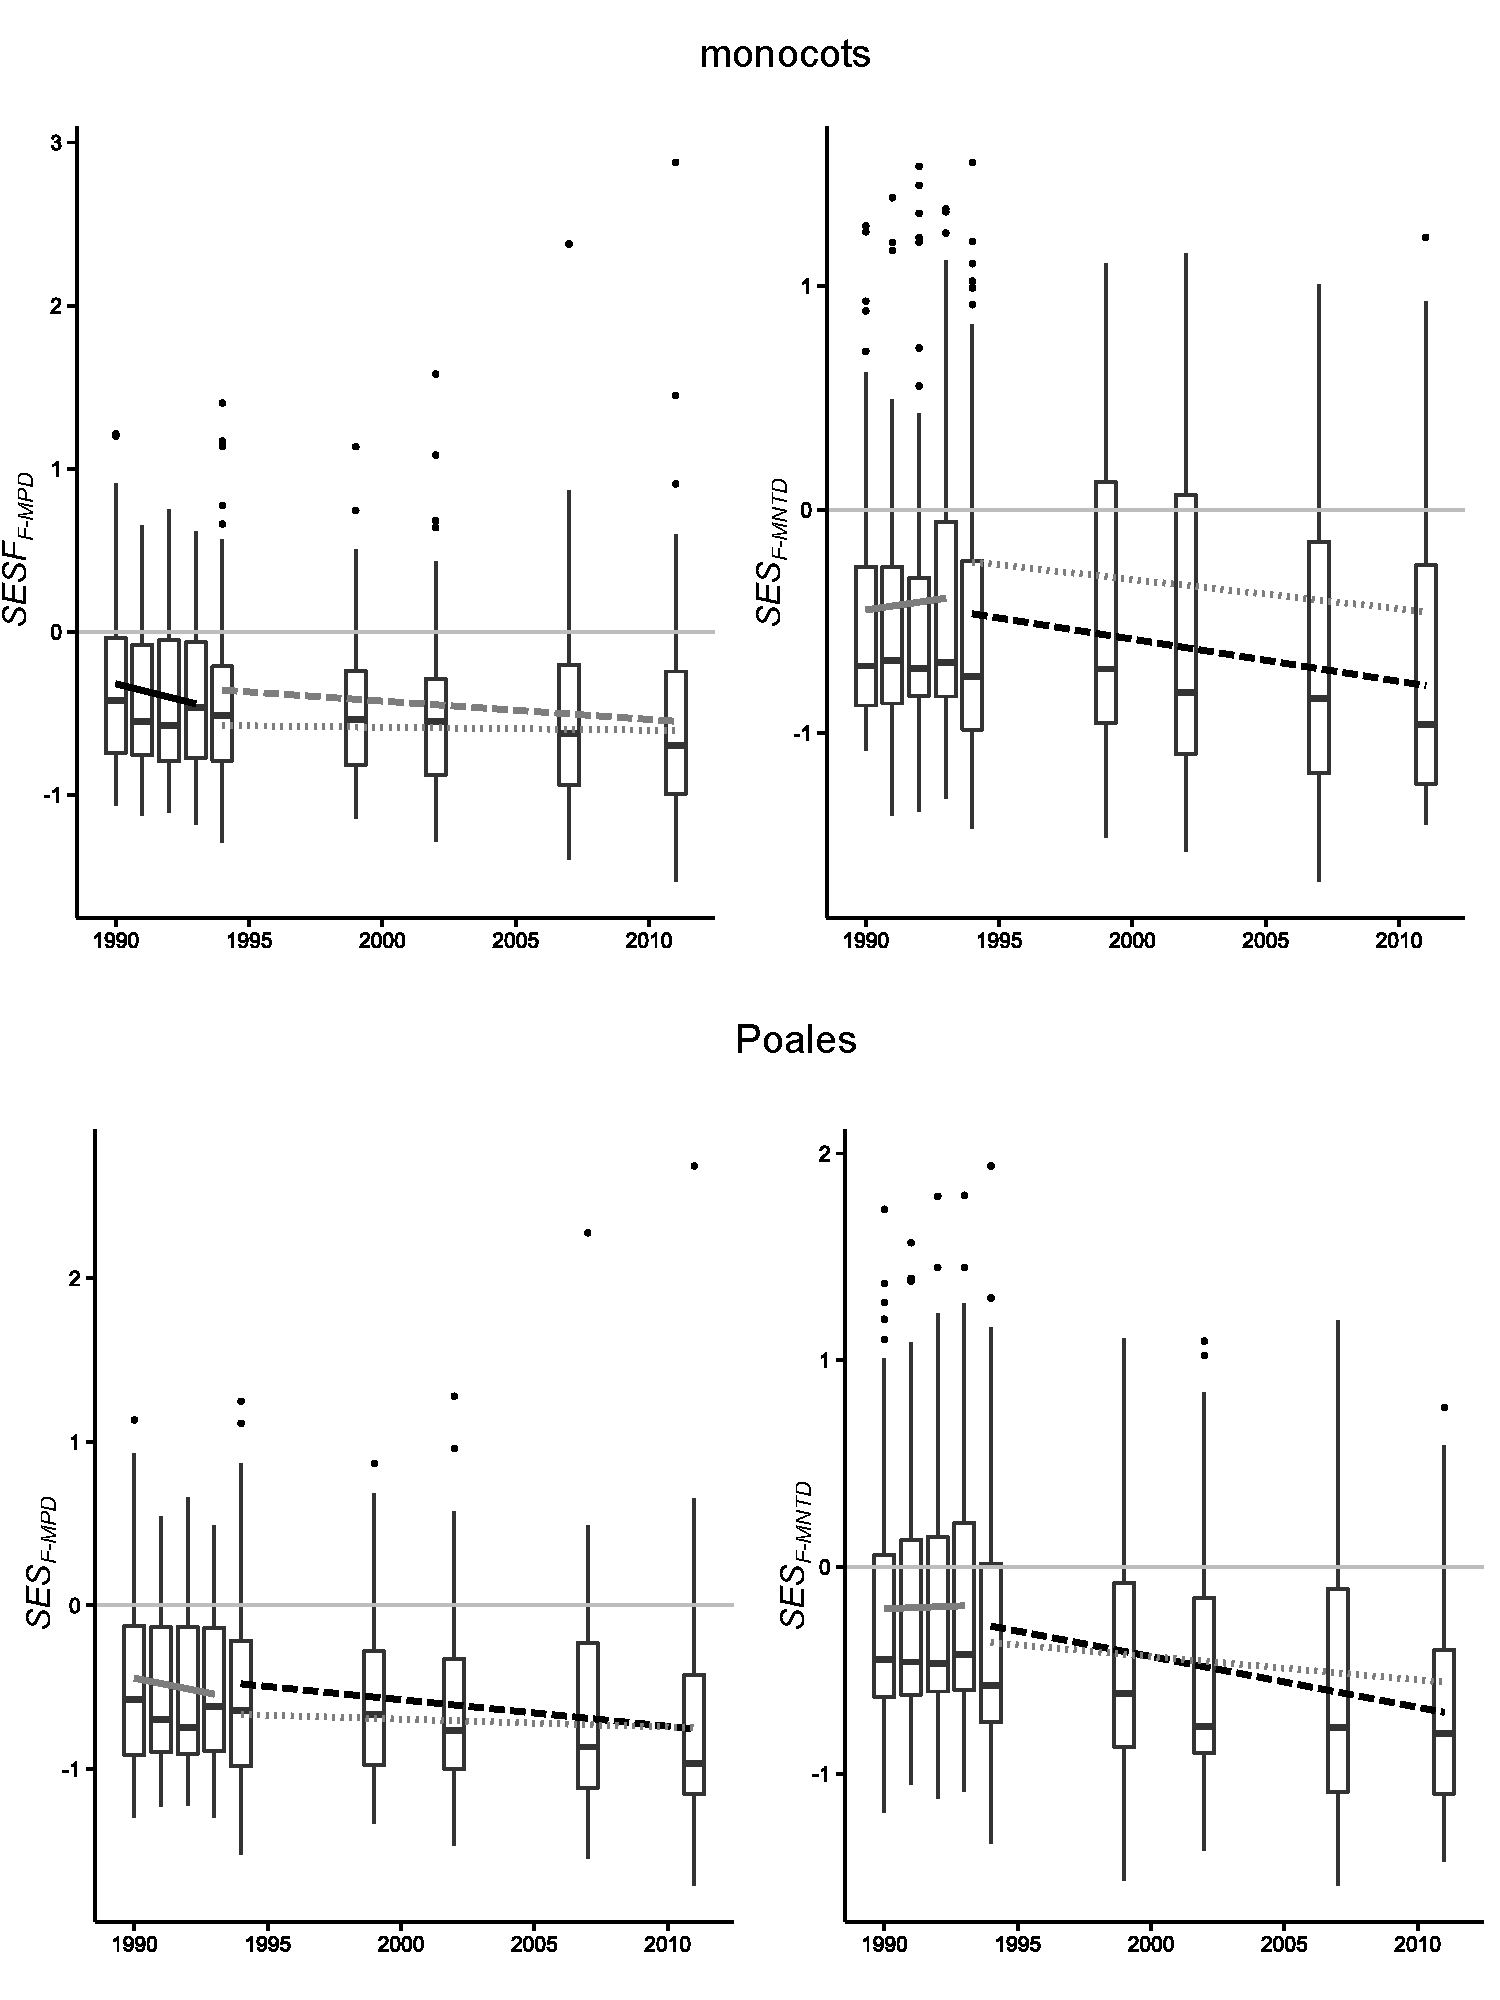
\includegraphics[width=0.7\linewidth]{func_poales_mono_alphadiv}\\
\footnotesize Figure S4.3. Functional community structure of monocots and Poales through time at the plot scale.
\end{figure}

\begin{figure}[H]
\centering
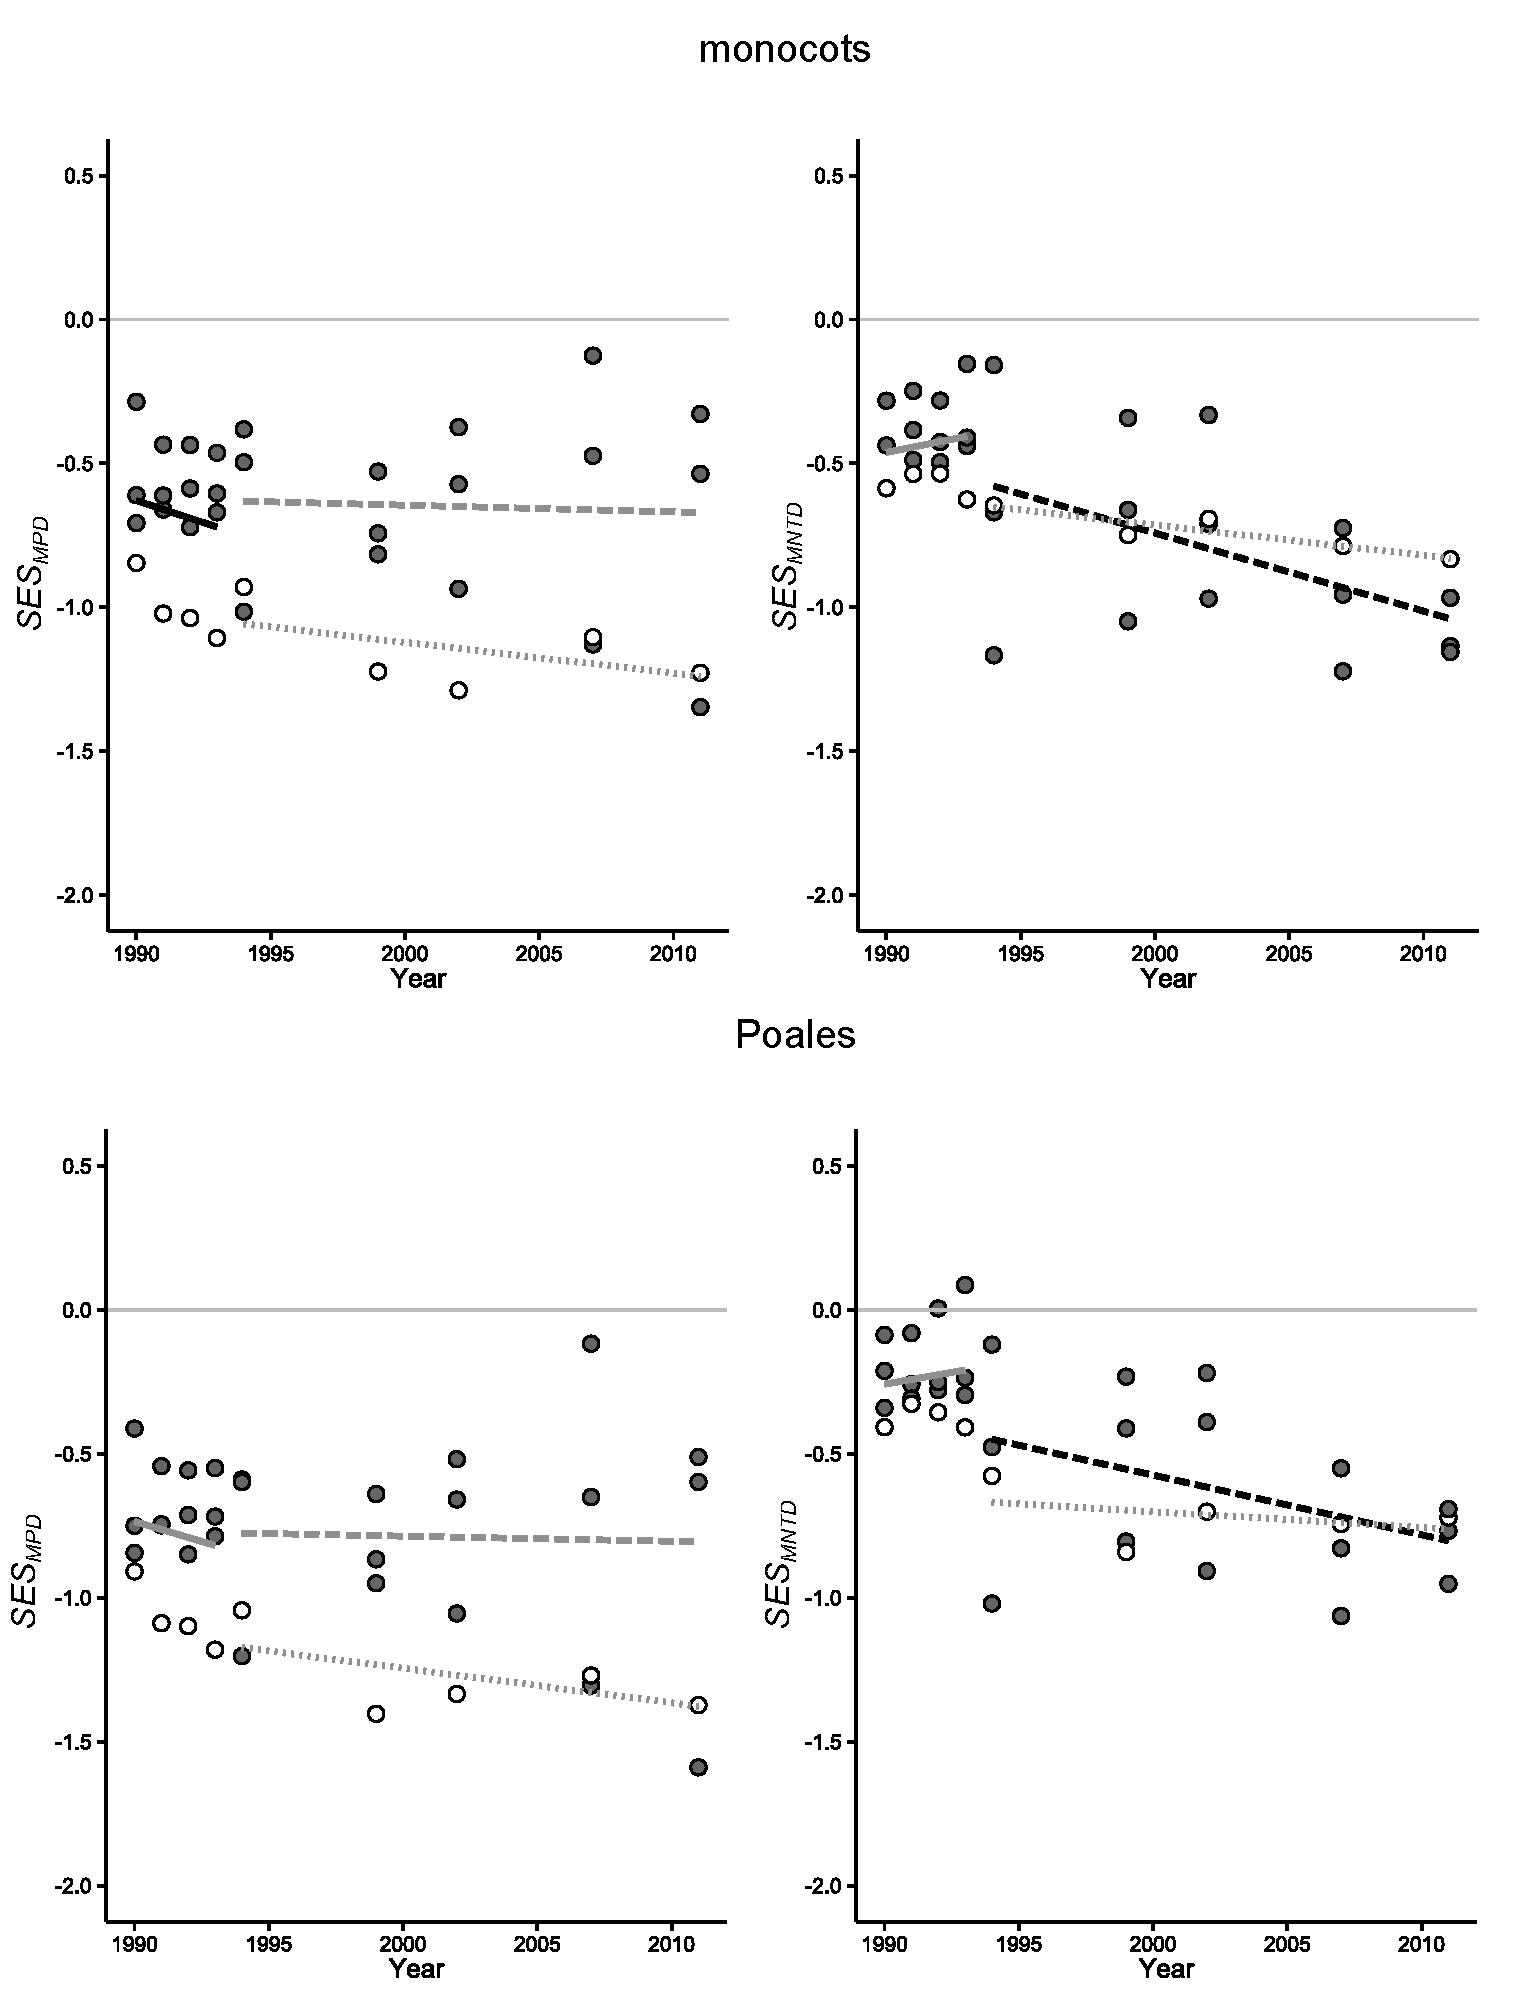
\includegraphics[width=0.7\linewidth]{func_alphadiv_poales_mono_scatter_transectscale}\\
\footnotesize Figure S4.4. Functional community structure of monocots and Poales through time at the site scale.
\end{figure}

\clearpage

\section{Temporal phylogenetic and functional beta turnover: supp. figs.}
\sectionmark{Temporal beta turnover: supp. figs.}

\begin{figure}[H]
\centering
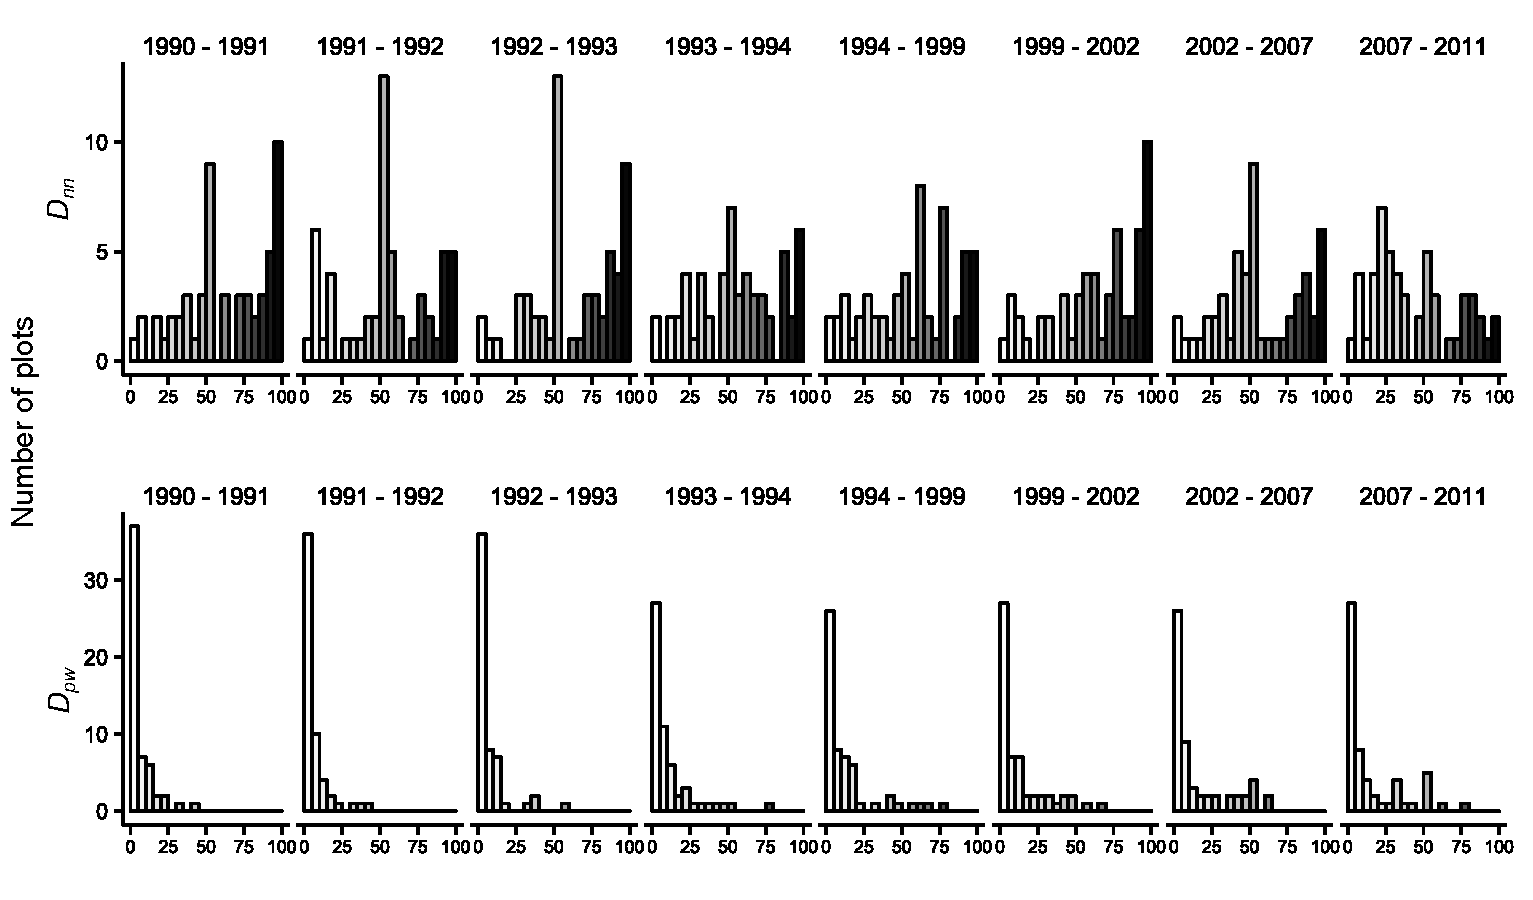
\includegraphics[width=1.0\linewidth]{full_phybeta_int}\\
\footnotesize Figure S4.5. Temporal phylogenetic beta turnover quantified by \textit{D}$_{nn}$ and  \textit{D}$_{pw}$ relative to the immediately preceding census point. Low quantile scores (white) indicate low turnover in phylogenetic composition relative to the observed rate of taxonomic turnover; high quantile scores (black) indicate high turnover in phylogenetic composition relative to the observed rate of taxonomic turnover. Values $<$2.5 or $>$97.5 are significant at the 0.05 level.
\end{figure}

\begin{figure}[H]
\centering
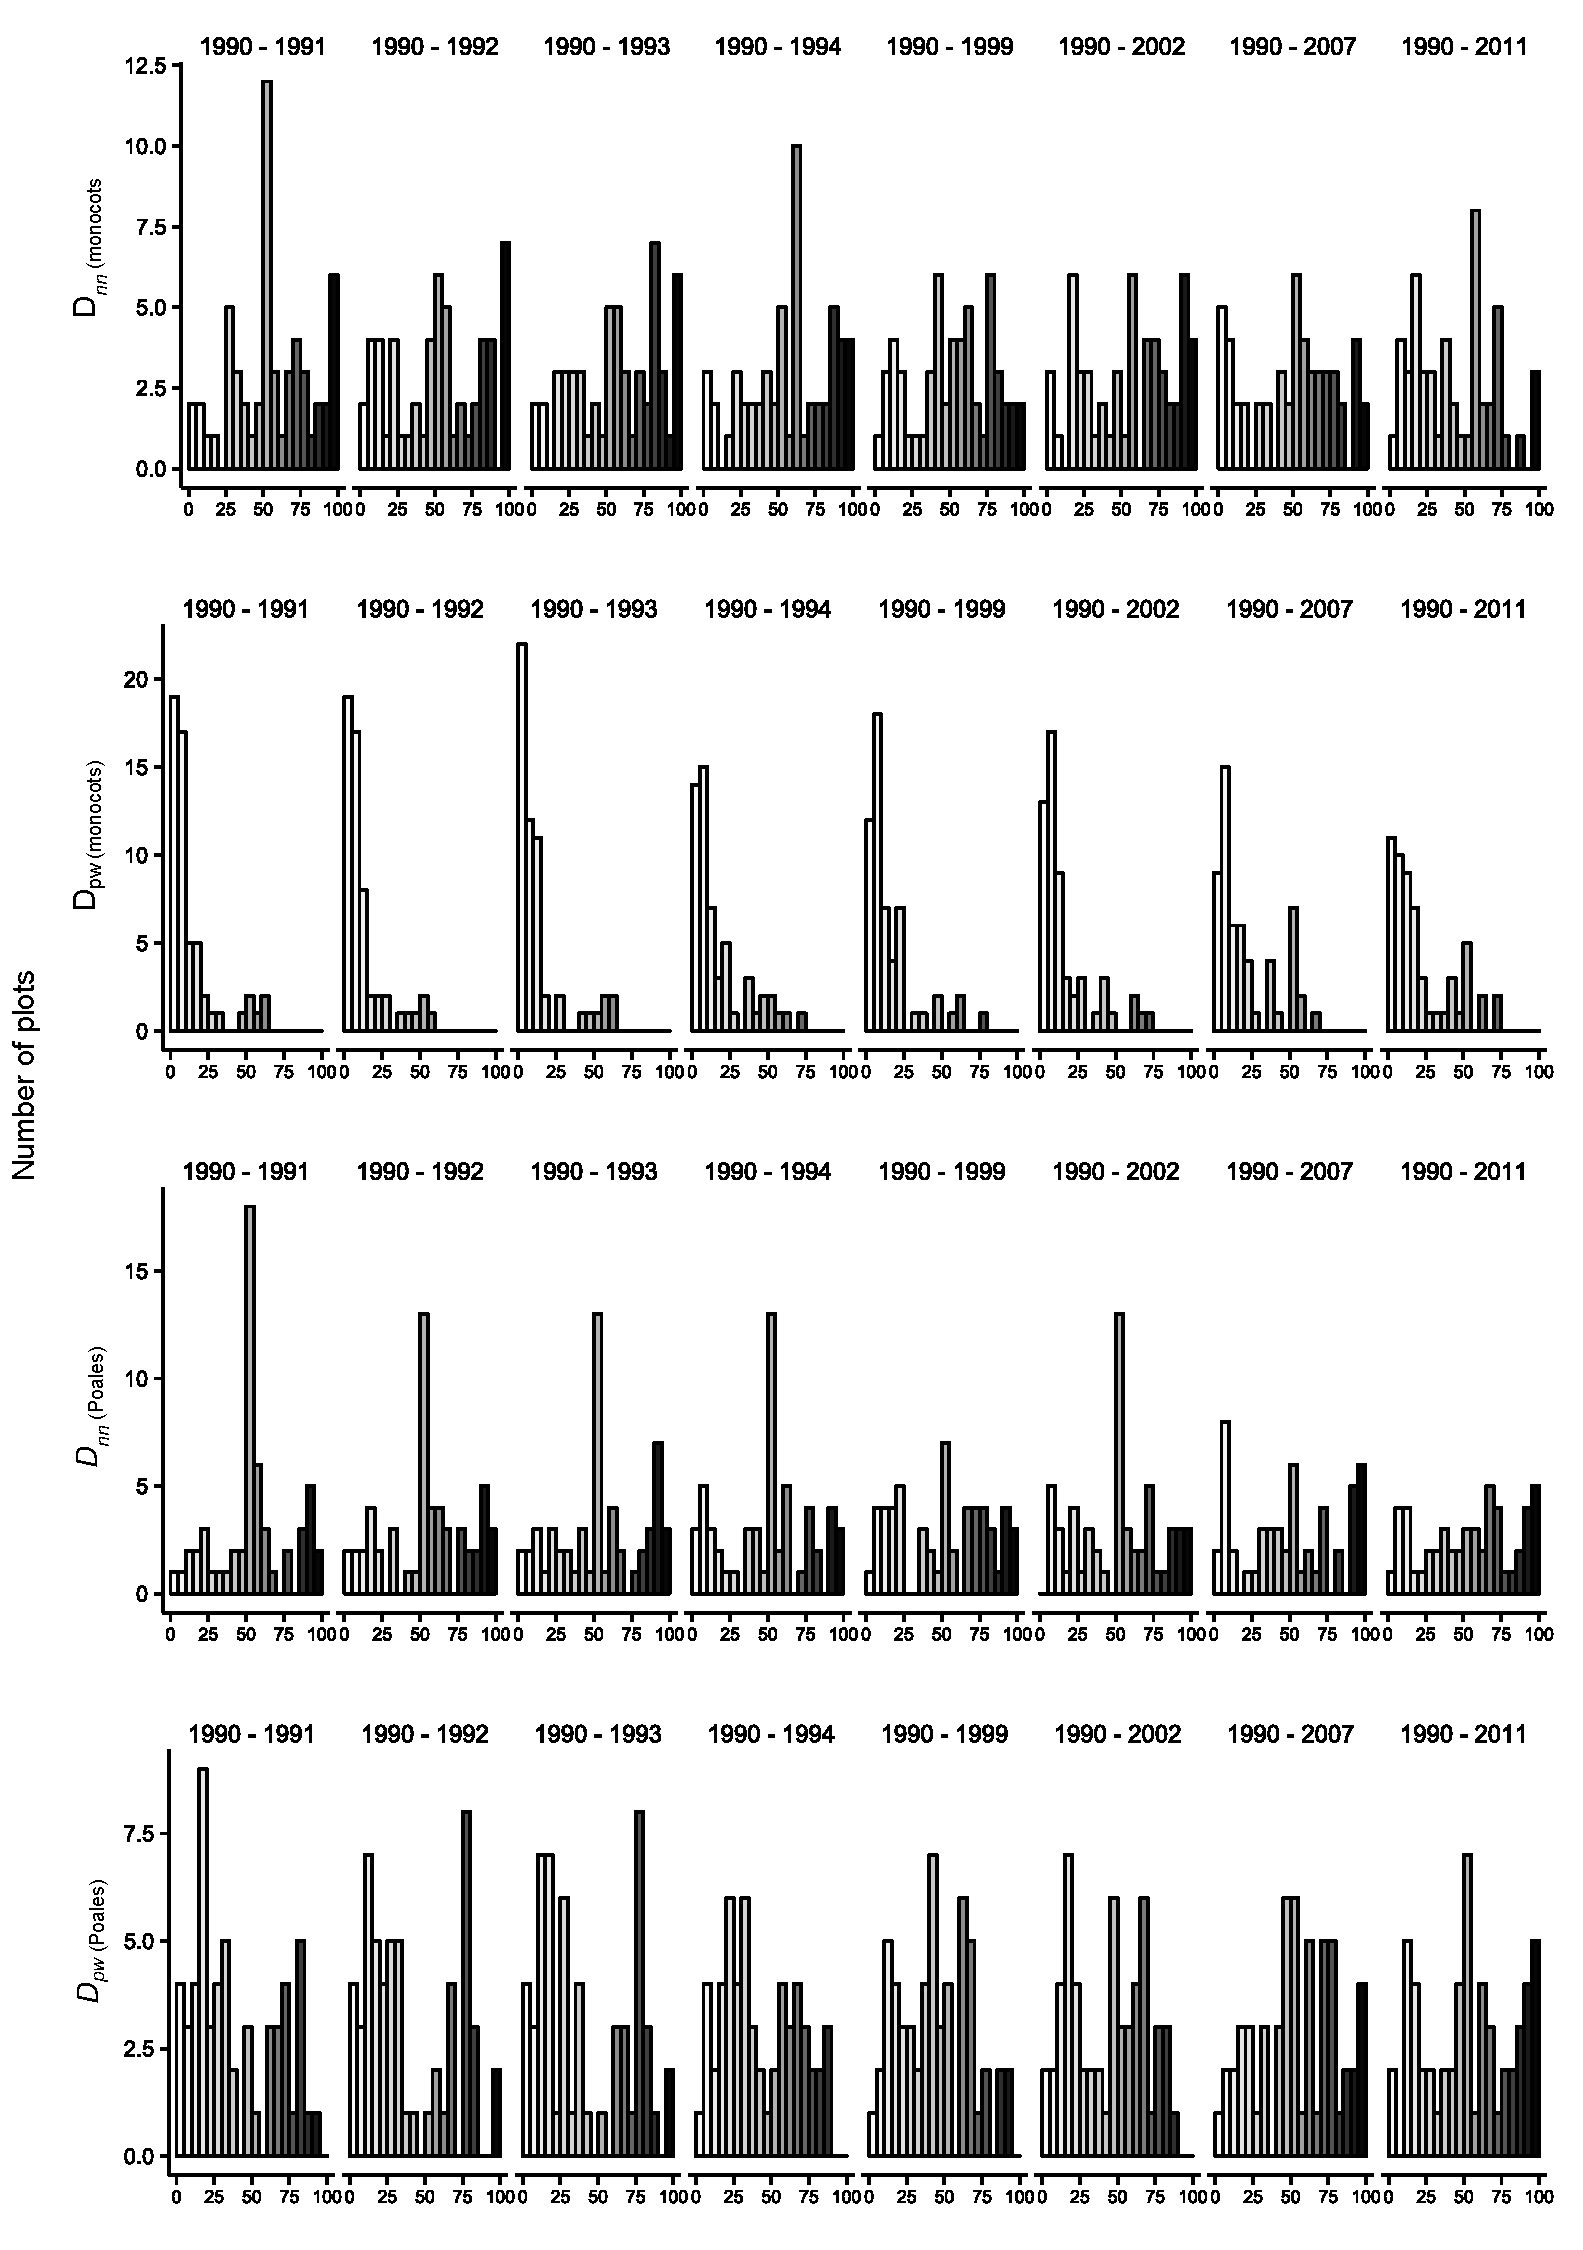
\includegraphics[width=0.8\linewidth]{mono_poales_phybeta}\\
\footnotesize Figure S4.6. Temporal phylogenetic beta turnover (monocots and Poales) quantified by \textit{D}$_{nn}$ and \textit{D}$_{pw}$ relative to the first census point. Low quantile scores (white) indicate low turnover in phylogenetic composition relative to the observed rate of taxonomic turnover; high quantile scores (black) indicate high turnover in phylogenetic composition relative to the observed rate of taxonomic turnover. Values $<$2.5 or $>$97.5 are significant at the 0.05 level.
\end{figure}


\begin{figure}[H]
\centering
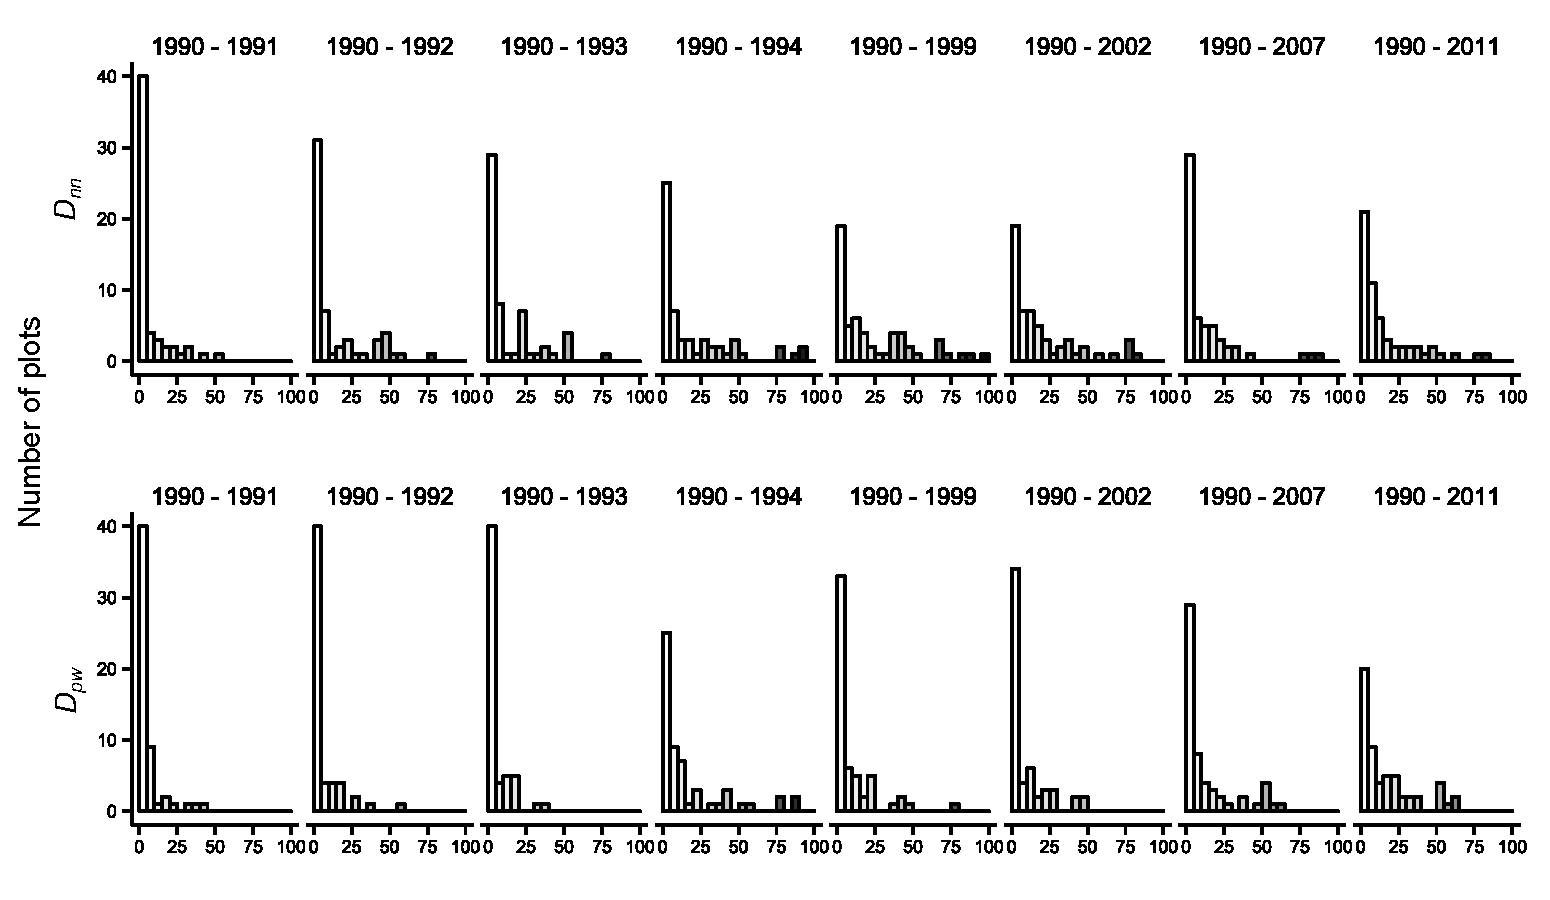
\includegraphics[width=1.0\linewidth]{full_funcbeta}\\
\footnotesize Figure S4.7. Temporal functional beta turnover quantified by \textit{D}$_{nn}$ and  \textit{D}$_{pw}$ relative to the first census point. Low quantile scores (white) indicate low turnover in phylogenetic composition relative to the observed rate of taxonomic turnover; high quantile scores (black) indicate high turnover in phylogenetic composition relative to the observed rate of taxonomic turnover. Values $<$2.5 or $>$97.5 are significant at the 0.05 level.
\end{figure}



\begin{figure}[H]
\centering
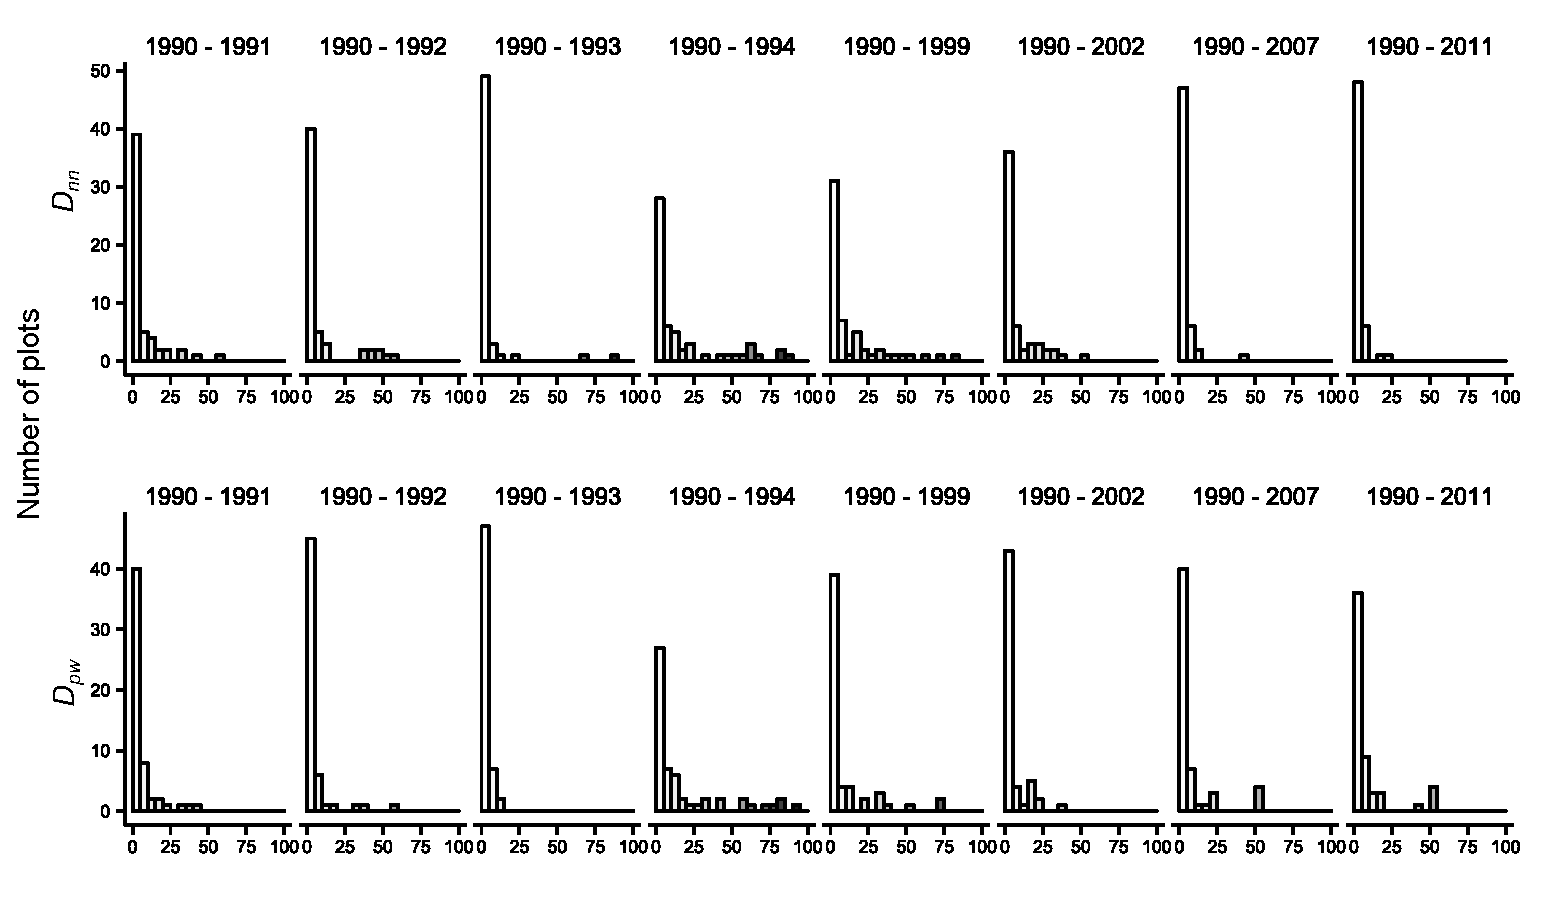
\includegraphics[width=1.0\linewidth]{full_funcbeta_int}\\
\footnotesize Figure S4.8. Temporal functional beta turnover quantified by \textit{D}$_{nn}$ and  \textit{D}$_{pw}$ relative to the immediately preceding census point. Low quantile scores (white) indicate low turnover in phylogenetic composition relative to the observed rate of taxonomic turnover; high quantile scores (black) indicate high turnover in phylogenetic composition relative to the observed rate of taxonomic turnover. Values $<$2.5 or $>$97.5 are significant at the 0.05 level.
\end{figure}

\begin{figure}[H]
\centering
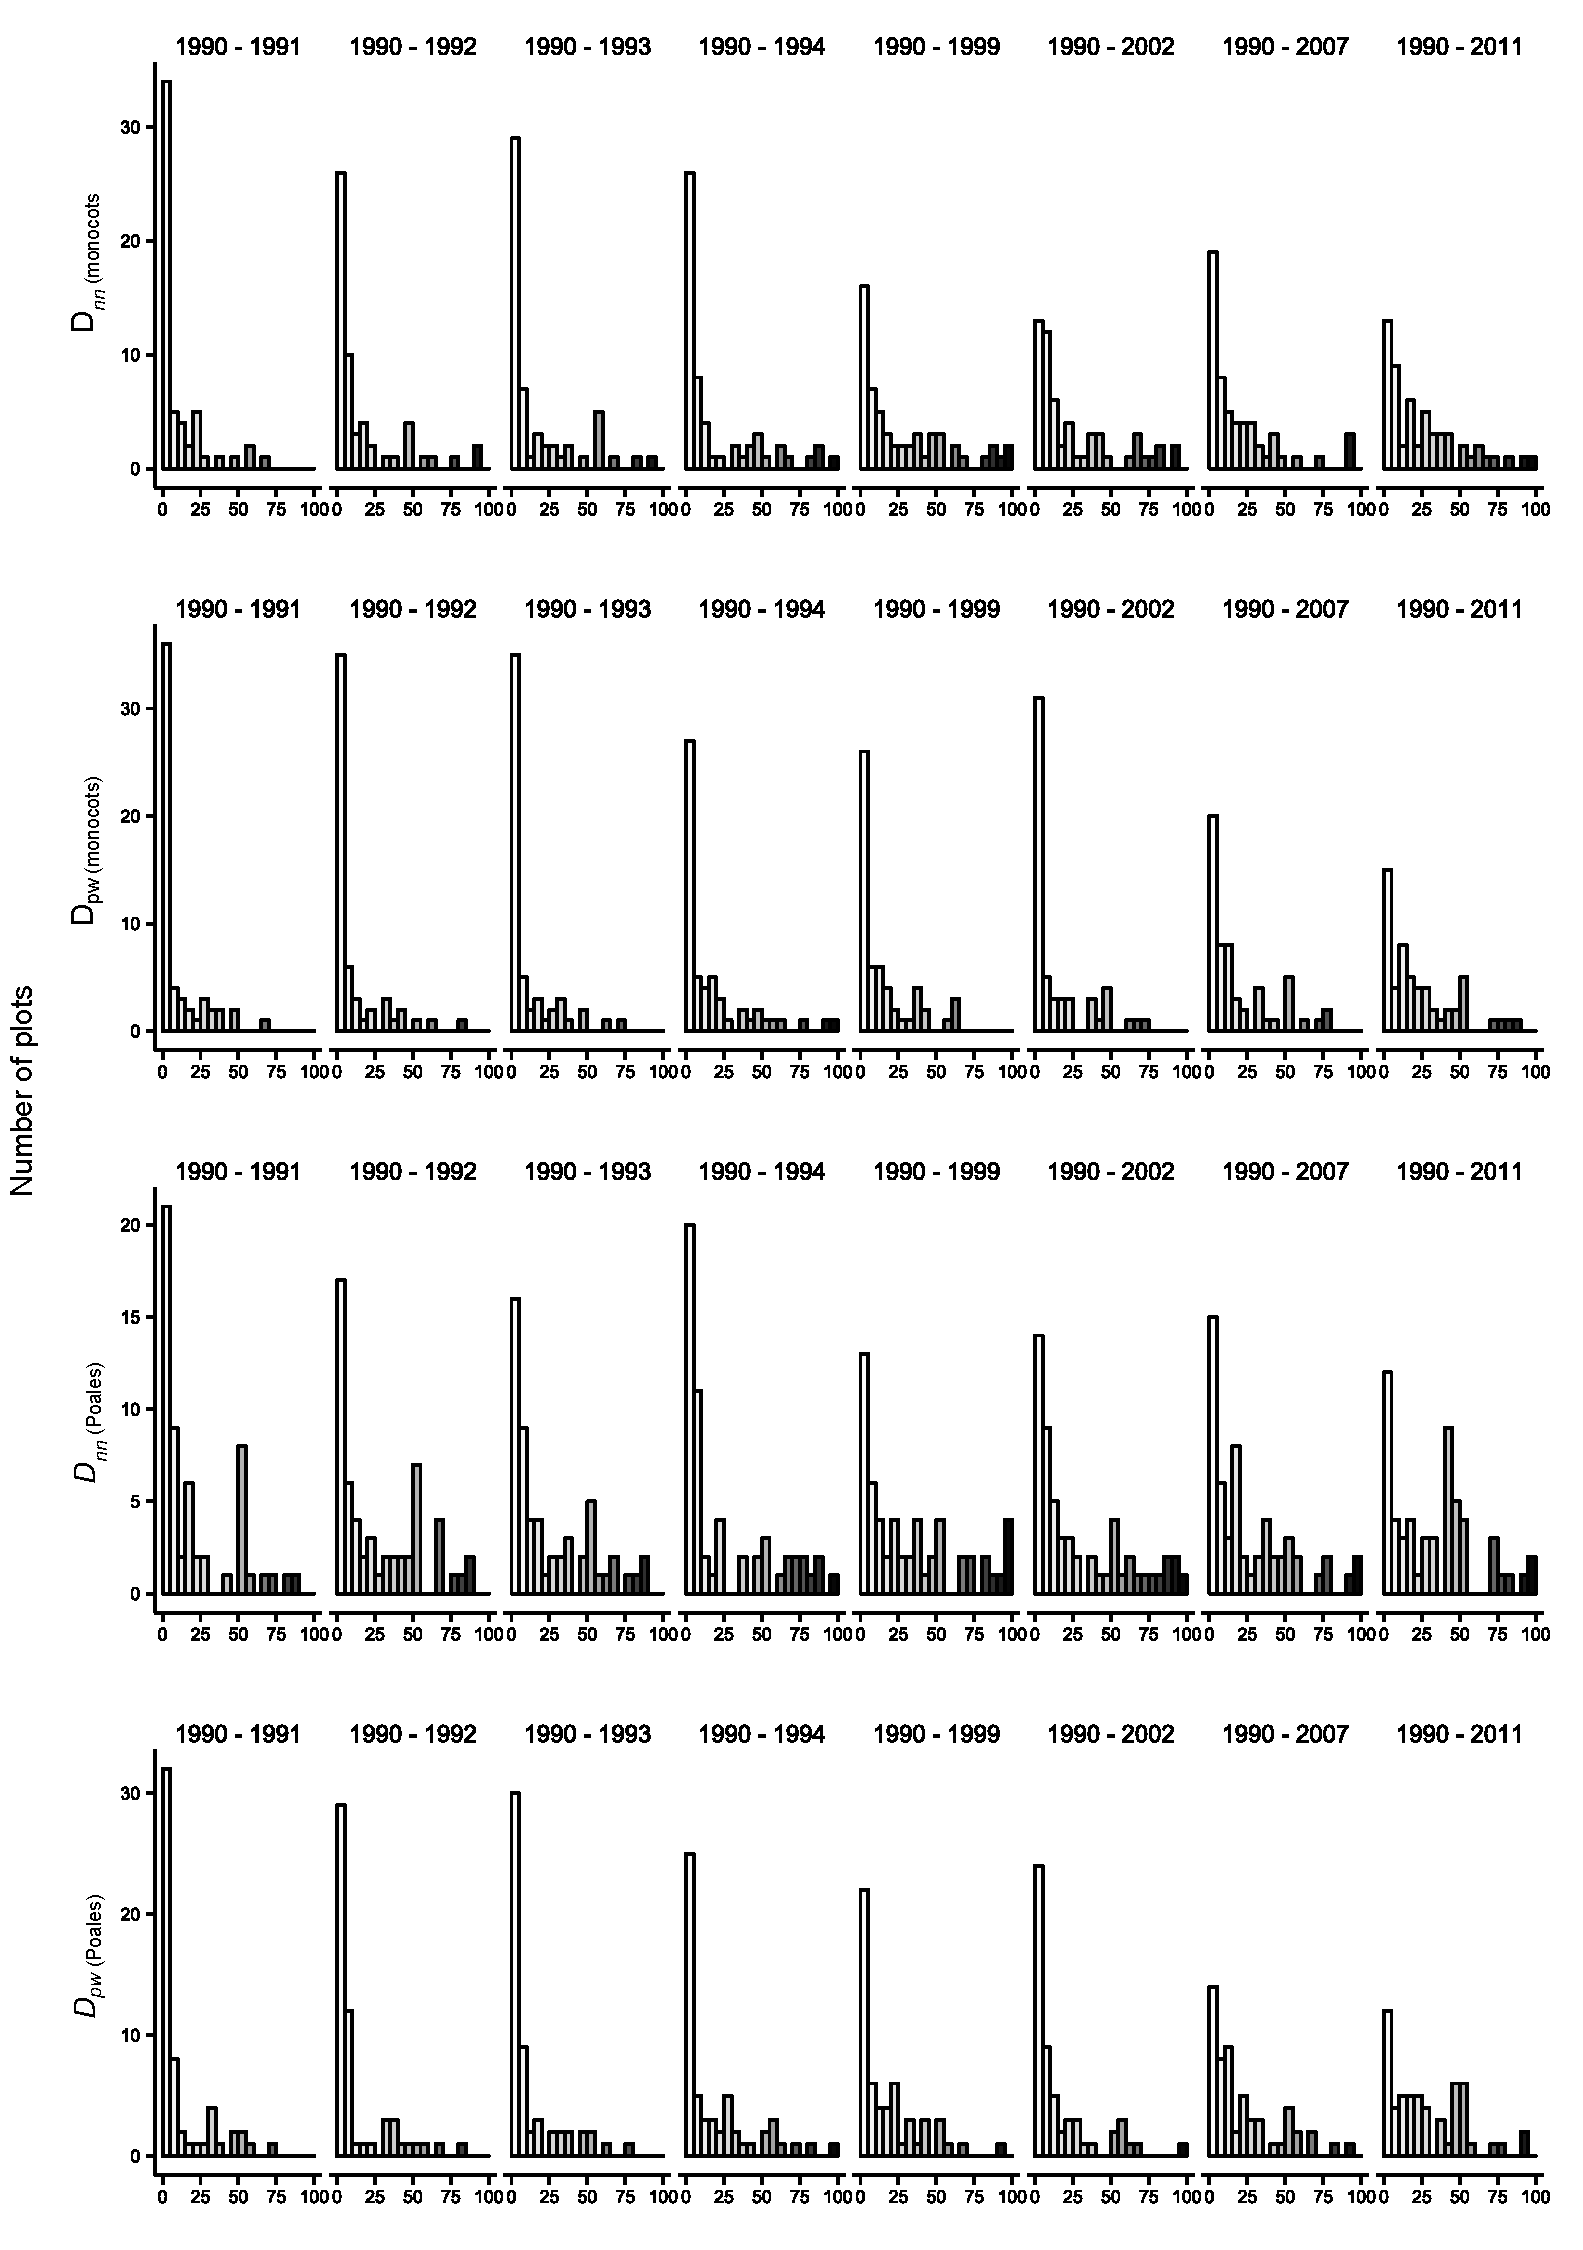
\includegraphics[width=0.8\linewidth]{mono_poales_funcbeta}\\
\footnotesize Figure S4.9. Temporal functional beta turnover (monocots and Poales) quantified by \textit{D}$_{nn}$ and \textit{D}$_{pw}$ relative to the first census point. Low quantile scores (white) indicate low turnover in phylogenetic composition relative to the observed rate of taxonomic turnover; high quantile scores (black) indicate high turnover in phylogenetic composition relative to the observed rate of taxonomic turnover. Values $<$2.5 or $>$97.5 are significant at the 0.05 level.
\end{figure}

\section{Species accumulation curve}

\begin{figure}[H]
\centering
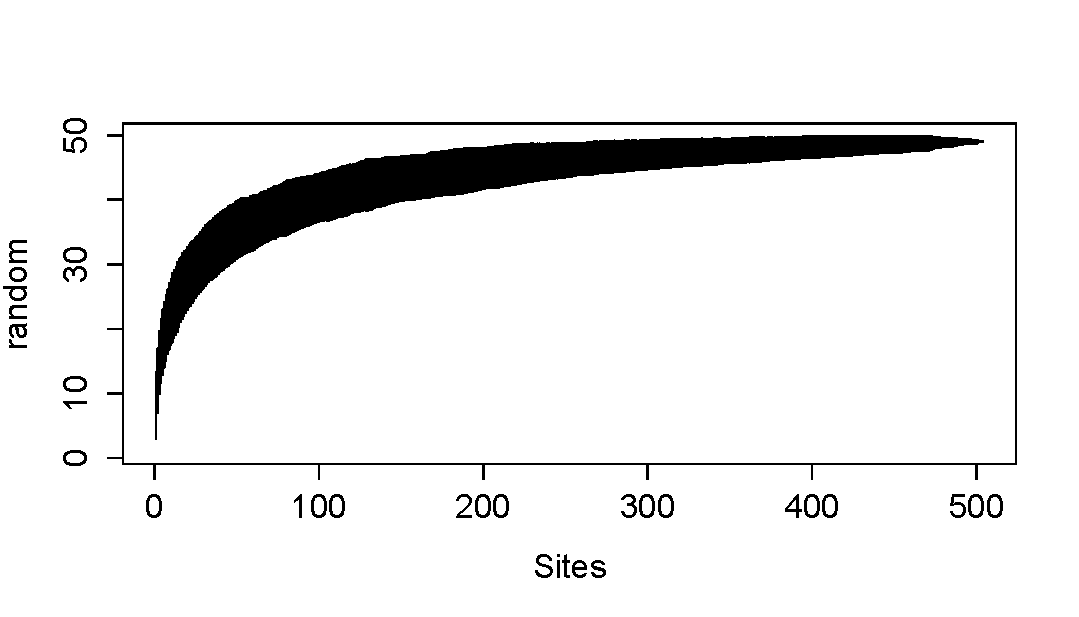
\includegraphics[width=1.0\linewidth]{sppaccum-sites}\\
\footnotesize Figure S4.10. Species accumulation curve obtained from 100 permutations of site in random order. Width denotes standard error.
\end{figure}

